\subsection{Überprüfung der Stabilität}
Zur Überprüfung der Stabilitätsbedingung \eqref{eq:Stabilitat} werden die Messwerte normiert, sodass die höchste Intensität jeweils den Wert 1 zugewiesen bekommt. Die resultierenden, sowie die gemessenen Werte sind in den Tabellen \ref{tab:curv} und \ref{tab:flat} zu sehen. Dann wird für den Resonator mit den beiden konkaven Spiegeln ein quadratisches Polynom -- in Anlehnung an \eqref{eq:StabCurv} -- an die Messwerte für die normierten Intensitäten gefittet. Das Ergebnis ist in Abbildung \ref{fig:fitcurved} dargestellt. Dasselbe wird mit den Werten für den Resonator mit einem flachen Spiegel und einer linearen Funktion gemacht. Die Ergebnisse hierfür finden sich in Abbildung \ref{fig:fitflat}. Auf die Angabe der errechneten Parameter wird hier verzichtet, da die gefittete Funktion offensichtlich weit von den Erwartungen abweicht.
\begin{table}
    \centering
    \caption{Resonatorlänge und dazu gemessene Intensität bei einem Resonator mit zwei konkaven Spiegeln}
    \label{tab:curv}
    \sisetup{parse-numbers=false}
    \begin{tabular}{
	S[table-format=1.2]
	S[table-format=3.0]
	}
	\toprule
	{$L \ / \ \mathrm{in} \si{\metre}$}		& {$I \ / \ \si{\micro\ampere}$}		\\ 
	\midrule
    0.6 & 177.0 & 0.3 \\
0.8 & 440.0 & 0.8 \\
0.9 & 530.0 & 0.9 \\
1.1 & 530.0 & 0.9 \\
1.2 & 350.0 & 0.6 \\
1.4 & 330.0 & 0.6 \\
1.6 & 440.0 & 0.8 \\
1.7 & 570.0 & 1.0 \\
1.9 & 500.0 & 0.9 \\
2.1 & 450.0 & 0.8 \\

    \bottomrule
    \end{tabular}
    \end{table}

\begin{figure}[h!]
	\centering
	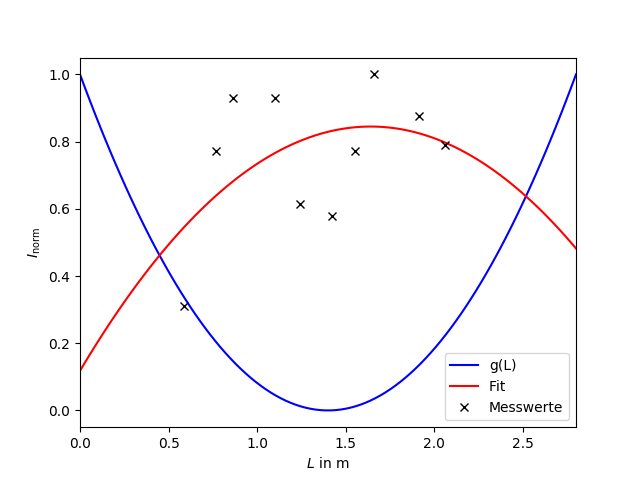
\includegraphics[width=.6\textwidth]{FitCurved.png}
	\caption{Fit zur Überprüfung der Stabilitätsbedingung bei zwei konkaven Spiegeln mit den Messwerten und der theoretisch erwarteten Funktion $g(L)$}
	\label{fig:fitcurved}
\end{figure}
\begin{table}
    \centering
    \caption{Resonatorlänge und dazu gemessene Intensität bei einem Resonator mit einem flachen und einem konkaven Spiegel}
    \label{tab:flat}
    \sisetup{parse-numbers=false}
    \begin{tabular}{
	S[table-format=1.2]
	S[table-format=3.0]
	}
	\toprule
	{$L \ / \ \mathrm{in} \si{\metre}$}		& {$I \ / \ \si{\micro\ampere}$}		\\ 
	\midrule
    0.5 & 20.0  & 0.1 \\
0.6 & 20.0  & 0.1 \\
0.7 & 39.0  & 0.3 \\
1.0 & 95.0  & 0.6 \\
0.9 & 104.0 & 0.7 \\
1.0 & 150.0 & 1.0 \\

    \bottomrule
    \end{tabular}
    \end{table}

\begin{figure}[h!]
	\centering
	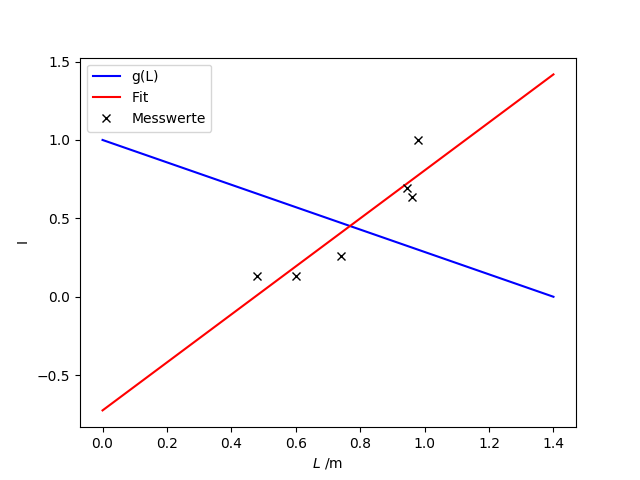
\includegraphics[width=.6\textwidth]{FitFlat.png}
	\caption{Fit zur Überprüfung der Stabilitätsbedingung bei einem gekrümmten und einem flachen Spiegel mit den Messwerten und der theoretisch erwarteten Funktion $g(L)$}
	\label{fig:fitflat}
\end{figure}